% !TeX root = ../proyecto.tex

\chapter{Desarrollo Experimental}\label{ch:desarrollo-experimental}
En este capítulo se exponen los experimentos realizados, los ajustes implementados en los algoritmos y los resultados
obtenidos en los distintos escenarios evaluados.
El objetivo principal fue analizar el rendimiento de los modelos entrenados con conjuntos de datos reducidos,
seleccionados mediante algoritmos meméticos y evolutivos.

\section{Datasets utilizados}\label{sec:datasets}
En el aprendizaje profundo, los datasets son colecciones de datos etiquetados o no etiquetados que se utilizan para
entrenar modelos.
Estos conjuntos de datos contienen ejemplos organizados que representan la entrada para el modelo y, en muchos casos,
también las etiquetas correspondientes que indican la salida deseada.
Los datasets varían en tamaño, calidad y tipo, dependiendo de la tarea a resolver, como la clasificación de imágenes,
el reconocimiento de patrones o la predicción de series temporales.


A continuación, se van a explicar cada uno de los Datasets que se han utilizado en el desarrollo del proyecto.

\newpage

\subsection{Rock, Paper, Scissors (Piedra, Papel, Tijera)}\label{subsec:rock-paper-scissors}
\textbf{Rock, Paper, Scissors}~\cite{RockPaperScissors} es un conjunto de datos creado por Laurence Moroney
que se utiliza para la clasificación de imágenes de manos representando los gestos de `piedra', `papel' y `tijeras'.

\begin{figure}[H]
    \centering
    \begin{subfigure}[t]{0.3\textwidth}
        \centering
        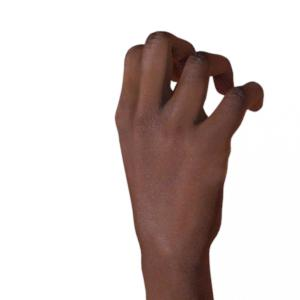
\includegraphics[width=\linewidth]{imagenes/dataset_examples/rock.jpg}
        \caption*{Rock}
    \end{subfigure}
    \begin{subfigure}[t]{0.3\textwidth}
        \centering
        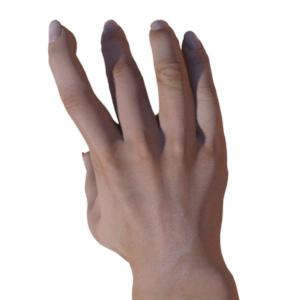
\includegraphics[width=\linewidth]{imagenes/dataset_examples/paper.jpg}
        \caption*{Paper}
    \end{subfigure}
    \begin{subfigure}[t]{0.3\textwidth}
        \centering
        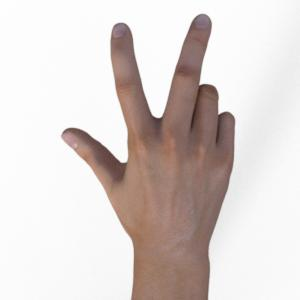
\includegraphics[width=\linewidth]{imagenes/dataset_examples/scissors.jpg}
        \caption*{Scissors}
    \end{subfigure}
    \caption{Ejemplos de imágenes del dataset Rock, Paper, Scissors}
    \label{fig:ejemplos-rps}
\end{figure}

En la figura~\ref{fig:ejemplos-rps} se han mostrado una imagen de cada una de las clases del dataset Rock, Paper, Scissors,
para que se pueda observar la similitud entre las distintas clases.

\subsubsection{Estructura del Dataset}
El conjunto de datos contiene aproximadamente 2,500 imágenes, distribuidas en tres categorías: piedra, papel y tijeras.
Las imágenes están en color y tienen un tamaño de 300x300 píxeles.

\begin{figure}[ht]
    \centering
    \begin{forest}mydirstyle
        [RPS
            [train
                    [rock
                            [image1.jpg]
                            [image2.jpg]
                            [\dots]
                    ]
                    [paper
                            [image1.jpg]
                            [image2.jpg]
                            [\dots]
                    ]
                    [scissors
                            [image1.jpg]
                            [image2.jpg]
                            [\dots]
                    ]
            ]
            [test (originalmente valid)
                [rock]
                    [paper]
                    [scissors]
            ]
            [valid (originalmente test)
                [rock]
                    [paper]
                    [scissors]
            ]
        ]
    \end{forest}
    \caption{Estructura de carpetas del dataset Rock, Paper, Scissors}
    \label{fig:estructura-rps}
\end{figure}


Como se puede observar en la Figura~\ref{fig:estructura-rps}, las imágenes están organizadas en directorios según su función en el entrenamiento
(entrenamiento, validación o prueba) y, dentro de cada partición, se dividen a su vez por clases del dataset.

\subsubsection{Formato de los Datos}
Las imágenes están en formato JPEG (\texttt{.jpg}).
Para su procesamiento, se han aplicado técnicas de preprocesamiento
adaptadas a los requerimientos del modelo.

\subsubsection{Uso del Dataset}
Este dataset se ha utilizado para evaluar el rendimiento del modelo en un problema de clasificación de imágenes con
múltiples clases, pero siendo un dataset sencillo y con un número de clases pequeño.
Además, permite explorar la eficacia de los algoritmos meméticos en un entorno más cercano al reconocimiento de objetos.

\subsubsection{Correcciones en la División de Datos}
Según la nota observada en el README del dataset:
\begin{quote}
    \textit{Note: in the source, Laurence calls ``validation'' as the ``test'', and ``test'' the ``validation''.}
\end{quote}
se han renombrado las particiones de \texttt{test} y \texttt{valid} para que correspondan correctamente con sus
propósitos.

\subsubsection{Licencia y uso}
Este conjunto de datos se distribuye bajo la licencia
\textbf{Creative Commons Attribution 4.0 International (CC BY 4.0)}, lo que permite su uso, modificación y distribución
con la condición de otorgar el crédito adecuado a los creadores originales~\cite{moroneyLaurenceMoroneyAI}.


\subsection{PAINTING (Art Images: Drawing/Painting/Sculptures/Engravings)}\label{subsec:painting}
El dataset \textbf{Art Images: Drawing/Painting/Sculptures/Engravings} es una colección de aproximadamente 9,000
imágenes organizadas en cinco categorías de arte: dibujos, pinturas, esculturas, grabados y arte iconográfico.

\begin{figure}[H]
    \centering
    \begin{subfigure}[t]{0.3\textwidth}
        \centering
        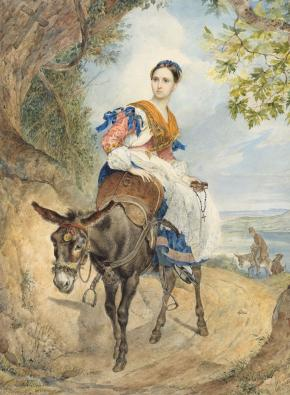
\includegraphics[width=\linewidth]{imagenes/dataset_examples/drawings.jpg}
        \caption*{Drawings}
    \end{subfigure}
    \begin{subfigure}[t]{0.3\textwidth}
        \centering
        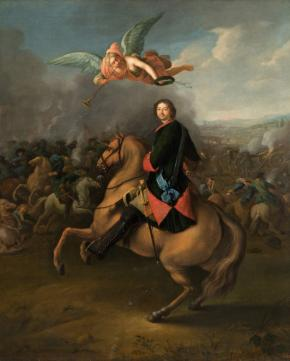
\includegraphics[width=\linewidth]{imagenes/dataset_examples/painting.jpg}
        \caption*{Painting}
    \end{subfigure}
    \begin{subfigure}[t]{0.3\textwidth}
        \centering
        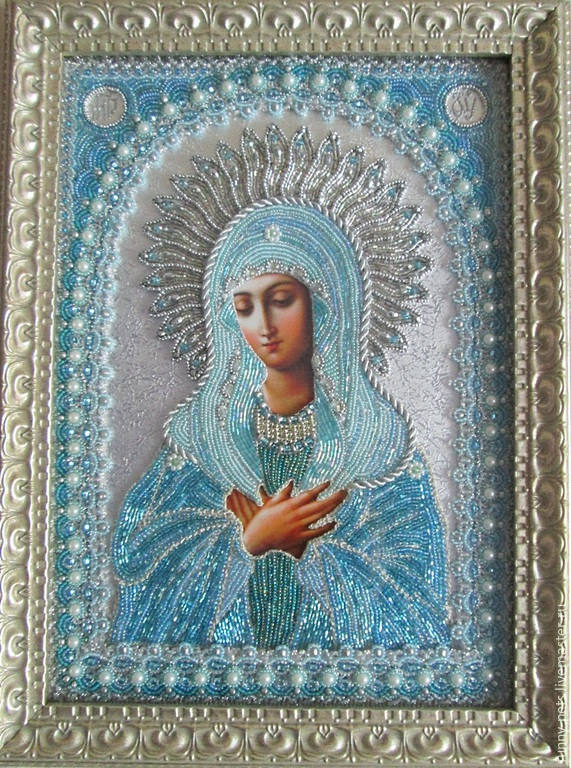
\includegraphics[width=\linewidth]{imagenes/dataset_examples/iconography.jpg}
        \caption*{Iconography}
    \end{subfigure}
    \begin{subfigure}[t]{0.3\textwidth}
        \centering
        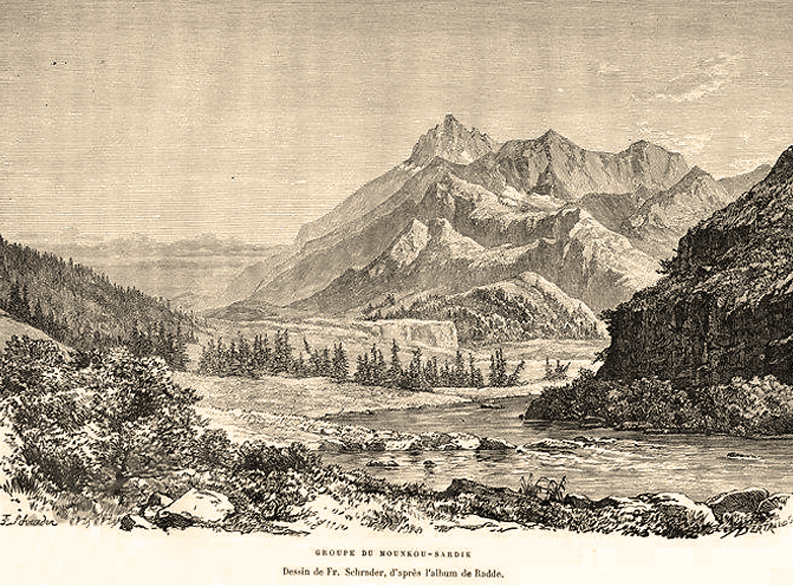
\includegraphics[width=\linewidth]{imagenes/dataset_examples/engraving.jpg}
        \caption*{Engraving}
    \end{subfigure}
    \begin{subfigure}[t]{0.3\textwidth}
        \centering
        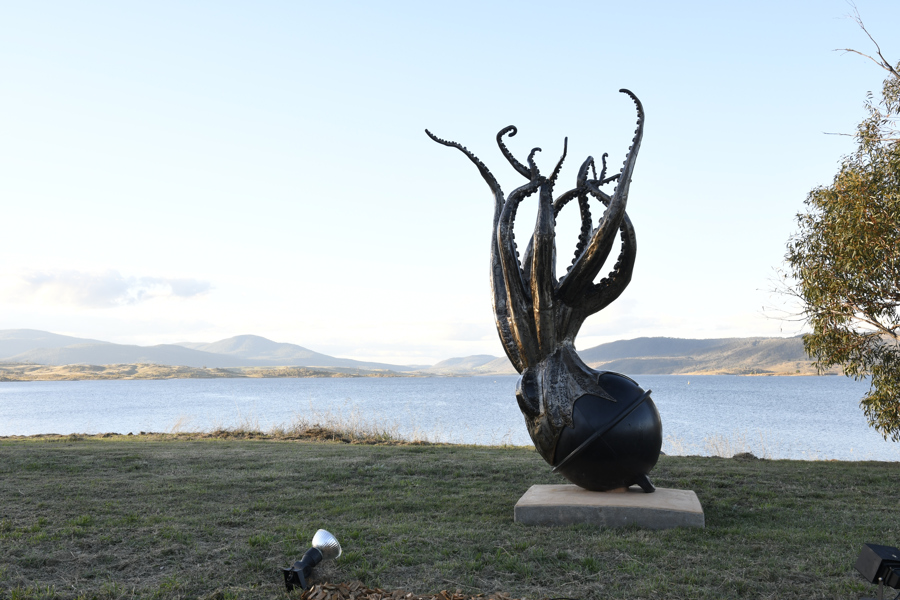
\includegraphics[width=\linewidth]{imagenes/dataset_examples/sculpture.jpg}
        \caption*{Sculpture}
    \end{subfigure}
    \caption{Ejemplos de clases en el dataset PAINTING}
    \label{fig:ejemplos-painting}
\end{figure}

En la figura~\ref{fig:ejemplos-painting} se han mostrado una imagen de cada una de las clases del dataset PAINTING,
para que se pueda observar la variabilidad de las imágenes.

\subsubsection{Estructura del Dataset}
\begin{figure}[ht]
    \centering
    \begin{forest}mydirstyle
        [Dataset
            [Train (originalmente training\_set)
                [drawings
                            [image1.jpg]
                            [image2.jpg]
                            [\dots]
                    ]
                    [paintings
                            [image1.jpg]
                            [image2.jpg]
                            [\dots]
                    ]
                    [sculptures]
                    [engravings]
                    [iconography]
            ]
            [Test (originalmente validation\_set)
                [drawings]
                    [paintings]
                    [sculptures]
                    [engravings]
                    [iconography]
            ]
        ]
    \end{forest}
    \caption{Estructura de carpetas del dataset PAINTING}
    \label{fig:estructura-painting}
\end{figure}

Como se puede observar en la Figura~\ref{fig:estructura-painting}, las imágenes están organizadas en directorios según su categoría artística,
que en este caso corresponden a las distintas clases del dataset, previamente divididas en conjuntos de entrenamiento y prueba.

\subsubsection{Formato de los Datos}
Todas las imágenes están en formato JPEG (\texttt{.jpg}) y presentan variaciones en resolución y dimensiones.
Se han aplicado técnicas de preprocesamiento para homogenizar las características de las imágenes.

\subsubsection{Uso del Dataset}
Este dataset se ha utilizado para entrenar y evaluar modelos de clasificación de imágenes en un entorno diferente al
RPS\@.
Con este dataset, se ha comprobado el funcionamiento para evaluar los algoritmos con un dataset un poco mas complejo
que el RPS, con un par de clases más y con un número mayor de imágenes.

\subsubsection{Correcciones en la División de Datos}
Observando los tamaños de la división de los datos, y teniendo en cuenta que la divisón de los datos suele ser en train
y test, se ha decidido por renombrar las particiones de \texttt{valid} por \texttt{test} para que corresponda
correctamente con su propósito.
Y el set de validation lo he obtenido separando el set de train, normalmente haciendo una división 80\% test y 20\%
valid.

\subsubsection{Acceso al Dataset}
Inicialmente, el dataset se descargó desde Kaggle~\cite{OriginalArtImages}

Sin embargo, debido a la presencia de archivos innecesarios y algunas imágenes corruptas, se optó por una versión
limpia disponible en Kaggle~\cite{CleanedArtImages}.

\subsubsection{Licencia y Uso}
Antes de su uso, se revisaron los términos y condiciones establecidos en la página de Kaggle para asegurar el
cumplimiento con las licencias y restricciones aplicables.

\subsection{Comparación entre datasets}\label{subsec:comparacion-entre-datasets}
A continuación, se muestra una tabla resumen con las características más relevantes de los datasets utilizados.
Esta comparación permite entender mejor la complejidad relativa de cada conjunto y cómo pueden influir en el comportamiento de los algoritmos:

\begin{table}[H]
    \centering
    \resizebox{\textwidth}{!}{
        \begin{tabular}{|l|c|c|c|c|}
            \hline
            \textbf{Dataset}      & \textbf{Nº Imágenes} & \textbf{Nº Clases} & \textbf{Formato} & \textbf{Tamaño Imagen} \\
            \hline
            Rock, Paper, Scissors & \textasciitilde2.500 & 3                  & JPG              & 300×300 px             \\
            PAINTING              & \textasciitilde9.000 & 5                  & JPG              & Variable               \\
            \hline
        \end{tabular}
    }
    \caption{Resumen comparativo de los datasets utilizados}
    \label{tab:resumen-datasets}
\end{table}

La selección de estos dos datasets responde a la necesidad de evaluar los algoritmos meméticos en distintos niveles de complejidad.
El dataset \textbf{Rock, Paper, Scissors} se utilizó en las primeras fases del proyecto como punto de partida,
ya que ofrecía un entorno sencillo y controlado, con un número reducido de clases y una estructura equilibrada.
Esto permitió desarrollar las bases del sistema y probar las primeras versiones de los algoritmos de manera más ágil y con menor complejidad computacional.

Por su parte, el dataset \textbf{PAINTING} se empleó posteriormente para validar el comportamiento de los algoritmos en un entorno más exigente.
Al incluir cinco categorías de arte con distintos estilos visuales, este conjunto introdujo una mayor variabilidad tanto semántica como estructural,
lo que permitió evaluar la robustez y capacidad de generalización de las soluciones desarrolladas.


\section{Diseño de los experimentos}\label{sec:diseño-de-los-experimentos}
La fase experimental se organizó en varias etapas.
Inicialmente se optó por un dataset simple (\textit{Rock, Paper, Scissors}) para validar el funcionamiento general del sistema.
Posteriormente, se realizaron pruebas con datasets más exigentes.
Los experimentos se repitieron utilizando diferentes porcentajes iniciales de datos (10\%, 25\%, 50\% y 75\%)
para estudiar cómo afecta la cantidad de datos seleccionados al rendimiento del modelo.

Con el fin de asegurar la consistencia entre ejecuciones experimentales, se aplicaron las medidas de control de reproducibilidad
descritas en el \hyperref[sec:consideraciones-de-optimizacion]{Apartado~\ref*{sec:consideraciones-de-optimizacion}}.
Esto permitió comparar algoritmos en condiciones homogéneas, evitando variaciones indeseadas causadas por componentes aleatorios del entorno de ejecución.

En cada prueba, se realizaron 5 ejecuciones en paralelo, cada una utilizando una semilla distinta.
Esta estrategia permitió obtener resultados promedio más robustos frente a la aleatoriedad del proceso evolutivo, asegurando una mayor fiabilidad estadística.

Los apartados siguientes explican con mayor detalle el procedimiento adoptado para llevar a cabo dichas ejecuciones.


\section{Procedimiento de Ejecución y Evaluación}\label{sec:procedimiento-de-ejecucion-y-evaluacion}
Para garantizar la consistencia y objetividad en la comparación entre algoritmos, se diseñó un procedimiento experimental sistemático y replicable.
Cada ejecución se realizó bajo las mismas condiciones computacionales y utilizando los mismos parámetros base,
salvo en aquellos casos en que se deseaba estudiar una variación concreta, como los distintos porcentajes iniciales o el uso de metaheurísticas con porcentajes libres.

\subsection{Métricas de Evaluación}\label{sec:metricas-de-evaluacion}
Para evaluar el rendimiento de los modelos se utilizaron métricas estándar como \textbf{accuracy}, \textbf{precisión}, \textbf{recall} y \textbf{F1-score},
calculadas sobre el conjunto de validación tras cada evaluación.
Para una definición formal de estas métricas, véase el \hyperref[sec:metricas-evaluacion]{Apartado~\ref*{sec:metricas-evaluacion}}.

Estas métricas fueron calculadas utilizando las funciones de \texttt{scikit-learn}, a partir de las predicciones del modelo y las etiquetas
reales correspondientes a los subconjuntos de imágenes seleccionados por cada algoritmo.

\subsection{Evaluaciones por Ejecución}\label{sec:evaluaciones-por-ejecucion}
Se buscó un equilibrio entre la cantidad de evaluaciones y el tiempo de ejecución, permitiendo una exploración suficiente del espacio de soluciones sin comprometer la eficiencia computacional.
Por ello, cada algoritmo fue configurado para realizar un máximo de 100 evaluaciones por ejecución,
independientemente del tipo de algoritmo utilizado, con el fin de mantener la equidad comparativa.

Cada evaluación consistía en generar un subconjunto de datos, entrenar el modelo correspondiente (ResNet50 o MobileNetV2),
y calcular su \textit{fitness} de acuerdo con las métricas mencionadas.

El número de evaluaciones sin mejora también fue monitorizado para aplicar criterios de parada anticipada,
explicados previamente en el \hyperref[sec:consideraciones-de-optimizacion]{Apartado~\ref*{sec:consideraciones-de-optimizacion}},
reduciendo así el tiempo computacional en caso de estancamiento.

\subsection{Repeticiones y Semillas}\label{sec:repeticiones-y-semillas}
Con el objetivo de obtener resultados estadísticamente significativos y reducir el efecto de la aleatoriedad,
cada configuración experimental fue ejecutada 5 veces, utilizando 5 semillas distintas.
Los resultados presentados en las tablas y gráficos corresponden a la media de esas ejecuciones,
junto con medidas de dispersión cuando procede, como los boxplots.

Cabe destacar que, en el caso de los boxplots, en lugar de representar la media de las 5 ejecuciones por configuración,
se optó por incluir todos los valores individuales obtenidos con las distintas semillas.
Esta decisión permite visualizar una distribución más realista del comportamiento de cada algoritmo,
resaltando mejor la mediana, así como los valores máximos y mínimos alcanzados durante las ejecuciones.

\subsection{Tiempos de Ejecución}\label{sec:tiempos-de-ejecucion}
Cada evaluación implicaba entrenar un modelo desde cero, por lo que los tiempos de ejecución fueron considerables.
Por ejemplo, una ejecución completa con 100 evaluaciones podía tardar entre 30 minutos y 2 horas,
dependiendo del algoritmo y del modelo utilizado.

Los algoritmos más complejos, como el memético o las versiones con reinicio poblacional,
requerían un mayor tiempo de ejecución debido a las operaciones adicionales de mejora local o regeneración de población.


\section{Evaluación con el conjunto completo}\label{sec:evaluacion-con-el-conjunto-completo}
Como punto de partida, se evaluó el rendimiento de los modelos convolucionales entrenados con el 100\% del conjunto de datos.
Esta prueba sirve como referencia para contrastar los resultados obtenidos mediante las técnicas de reducción aplicadas posteriormente.
Se utilizó tanto ResNet50 como MobileNetV2, y se midieron métricas como accuracy, precisión, recall y F1-score sobre el conjunto de validación.

\begin{table}[htp]
    \centering
    \resizebox{\textwidth}{!}{
        \begin{tabular}{lp{2cm}lp{2cm}p{2cm}p{2cm}p{2cm}p{2.2cm}}
            \toprule
            \textbf{Porcentaje Inicial} & \textbf{Duración}     & \textbf{Accuracy (Avg)} &
            \textbf{Precision (Avg)}    & \textbf{Recall (Avg)} & \textbf{F1-score (Avg)} &
            \textbf{Evaluaciones Realizadas}                                                                                \\
            \midrule
            100                         & 00:02:42              & 87,90\%                 & 88,96\% & 87,90\% & 87,81\% & 1 \\
            \bottomrule
        \end{tabular}
    }
    \caption{Resultados de ResNet50 entrenado con el 100\% del conjunto de datos.}
    \label{tab:resultados-100-resnet50}
\end{table}

Los resultados en la tabla~\ref{tab:resultados-100-resnet50} obtenidos representan el rendimiento máximo alcanzable en condiciones ideales,
sin reducción de datos, lo que permite establecer un techo de rendimiento frente al cual comparar las demás técnicas.


\section{Evaluación del enfoque aleatorio}\label{sec:evaluacion-enfoque-aleatorio}
El segundo experimento consistió en aplicar una selección aleatoria de ejemplos para distintos porcentajes iniciales de datos (10\%, 25\%, 50\% y 75\%).
Este enfoque, descrito en el \hyperref[sec:algoritmo-aleatorio]{Apartado~\ref*{sec:algoritmo-aleatorio}}, sirvió como línea base para evaluar la eficacia de los enfoques metaheurísticos.

\begin{figure}[!h]
    \centering
    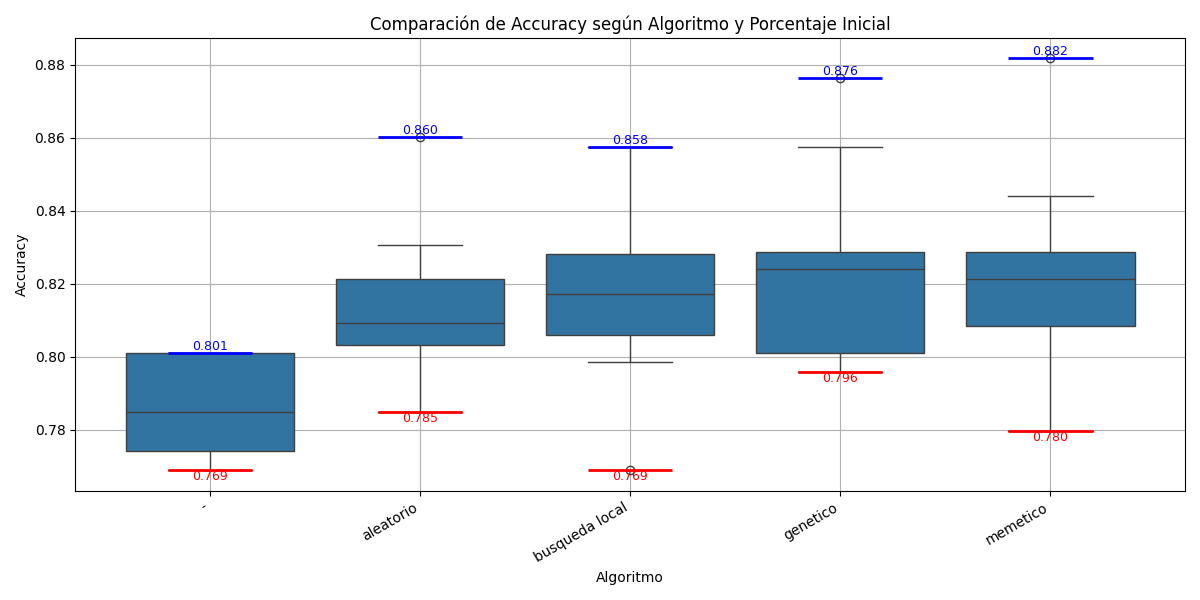
\includegraphics[width=0.95\textwidth]{imagenes/mobilenet-BOXPLOT-generacion-inicial}
    \caption{Boxplot comparando el \textit{accuracy} alcanzado por cada algoritmo de los iniciales.}
    \label{fig:resnet-boxplot-generacion-inicial}
\end{figure}

\colorbox{yellow}{Falta modificar la tabla~\ref{fig:resnet-boxplot-generacion-inicial} para que compare el 100\% con el aleatorio de resnet y ajustar analisis si es necesario.}
\colorbox{yellow}{Falta añadir tabla comparando resultados por porcentajes iniciales.}

Tal como se observa en el boxplot generado (\hyperref[fig:resnet-boxplot-generacion-inicial]{Figura~\ref*{fig:resnet-boxplot-generacion-inicial}}),
como era de esperar, presenta una alta dispersión, pero el rendimiento es mejor que el resultado con el 100\% del dataset.
Ademas, en esta otra tabla [tabla comparando resultados por porcentajes iniciales] los resultados mejoran de forma proporcional al incremento del porcentaje de imágenes seleccionadas.
Este comportamiento se justifica por la ausencia de una estrategia que guíe la selección de datos, lo que da lugar a conjuntos de entrenamiento inconsistentes y
resalta la necesidad de aplicar técnicas más sofisticadas para obtener resultados consistentes con menores volúmenes de datos.


\section{Comparación entre modelos convolucionales}\label{sec:comparacion-modelos-convolucionales}
Antes de analizar los algoritmos de reducción, se comparó el comportamiento de los modelos \textbf{ResNet50} y \textbf{MobileNetV2} bajo las mismas condiciones de entrenamiento y subconjuntos aleatorios.

\begin{table}[H]
    \centering
    \resizebox{\textwidth}{!}{
        \begin{tabular}{lp{2cm}lp{2cm}p{2cm}p{2cm}p{2cm}p{2.2cm}}
            \toprule
            \textbf{Algoritmo}       & \textbf{Porcentaje Inicial} & \textbf{Duración}       & \textbf{Accuracy (Avg)} &
            \textbf{Precision (Avg)} & \textbf{Recall (Avg)}       & \textbf{F1-score (Avg)} &
            \textbf{Evaluaciones Realizadas}                                                                                                               \\
            \midrule
            \multicolumn{8}{l}{\textbf{Modelo ResNet50}}                                                                                                   \\
            \midrule
            aleatorio                & 10                          & 00:45:08                & 76,55\%                 & 81,80\% & 76,55\% & 76,25\% & 100 \\
            aleatorio                & 20                          & 01:10:27                & 81,77\%                 & 84,70\% & 81,77\% & 81,59\% & 100 \\
            aleatorio                & 50                          & 02:24:49                & 87,14\%                 & 88,09\% & 87,14\% & 86,97\% & 100 \\
            aleatorio                & 100                         & 00:02:42                & 87,90\%                 & 88,96\% & 87,90\% & 87,81\% & 1   \\
            \midrule
            \multicolumn{8}{l}{\textbf{Modelo MobileNet}}                                                                                                  \\
            \midrule
            aleatorio                & 10\%                        & 00:29:29                & 72,31\%                 & 76,40\% & 72,31\% & 69,62\% & 100 \\
            aleatorio                & 20\%                        & 00:50:36                & 76,48\%                 & 78,82\% & 76,48\% & 75,58\% & 100 \\
            aleatorio                & 50\%                        & 01:54:09                & 75,56\%                 & 79,72\% & 75,56\% & 74,67\% & 100 \\
            -                        & 100\%                       & 00:03:16                & 78,60\%                 & 81,55\% & 78,60\% & 77,68\% & 1   \\
            \bottomrule
        \end{tabular}
    }
    \caption{Comparativa de resultados de la generación inicial utilizando el algoritmo \textbf{aleatorio} con los modelos \textbf{ResNet50} y \textbf{MobileNet}.}
    \label{tab:resnet50-vs-mobilenet}
\end{table}

Los resultados de la tabla~\ref{tab:resnet50-vs-mobilenet} muestran que ResNet50 mostró consistentemente mejores métricas,
aunque a costa de mayores tiempos de entrenamiento.
Por su parte, MobileNetV2 demostró ser más eficiente, resultando útil para entornos con restricciones computacionales.

Esta comparación justificó la elección de MobileNet como modelo principal en el resto de los experimentos,
dada su superior eficiencia en términos de tiempo y recursos, posibilitando la facilidad de realizar múltiples pruebas en un tiempo razonable.


\section{Estudio de la búsqueda local}\label{sec:estudio-busqueda-local}
Como se describió en el apartado correspondiente (ver \hyperref[sec:algoritmo-busqueda-local]{Sección~\ref*{sec:algoritmo-busqueda-local}}),
la búsqueda local permite mejorar progresivamente una solución inicial mediante pequeñas modificaciones guiadas por el rendimiento.
En este apartado se evalúa su efectividad como alternativa más estructurada frente al enfoque aleatorio, pero sin llegar a la complejidad de los algoritmos evolutivos.
Su inclusión busca analizar hasta qué punto una estrategia simple pero guiada puede generar subconjuntos de datos más representativos y consistentes.

\begin{figure}[H]
    \centering
    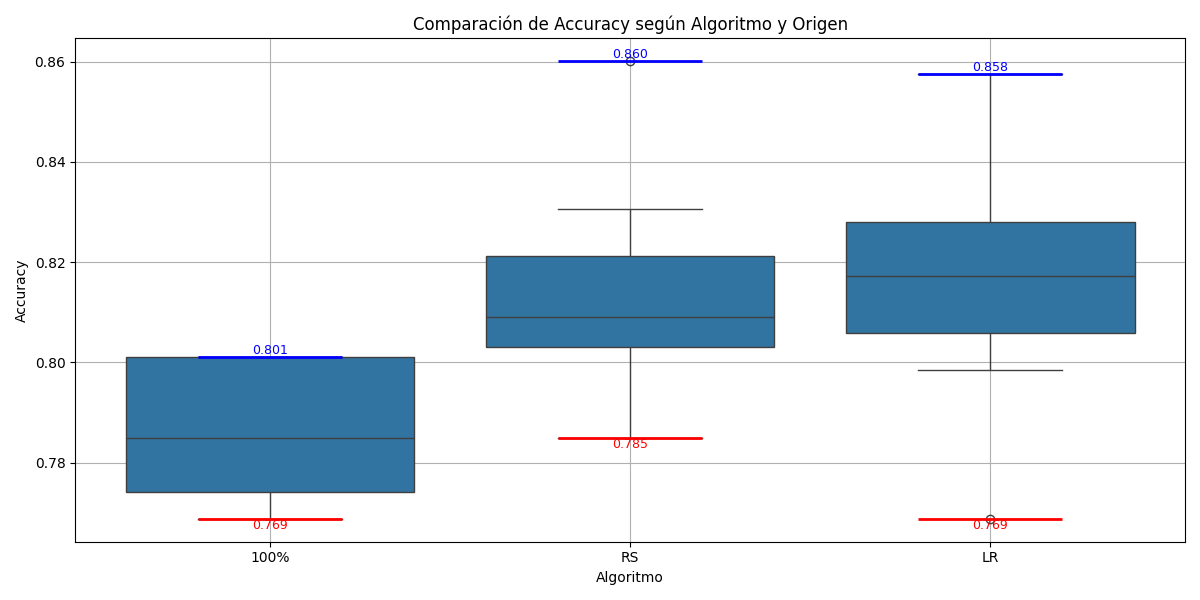
\includegraphics[width=1\textwidth]{imagenes/evaluaciones/comparacion_aleatorio-bl}
    \caption{Boxplot comparando el algoritmo aleatorio con la búsqueda local usando \textit{accuracy}.}
    \label{fig:aleatorio-vs-busqueda-local}
\end{figure}

En la Figura~\ref{fig:aleatorio-vs-busqueda-local} se muestran los resultados mediante un boxplot que permite observar
la distribución completa de valores obtenidos en las distintas ejecuciones.

Se puede apreciar que el algoritmo de búsqueda local mejora claramente la mediana del accuracy respecto al enfoque aleatorio.
Mientras que el enfoque aleatorio se sitúa en torno a una mediana de 0.787, la búsqueda local alcanza una mediana superior, próxima a 0.818.
Esta diferencia refleja una mayor capacidad del algoritmo local para generar subconjuntos más representativos y eficaces.

Además, los valores máximos alcanzados por ambos algoritmos son similares (en torno a 0.858-0.860),
pero la búsqueda local muestra una dispersión más acotada hacia valores altos, lo que sugiere mayor estabilidad en sus resultados.
En cambio, el algoritmo aleatorio presenta una mayor dispersión hacia valores bajos y una mayor sensibilidad a la aleatoriedad de las selecciones,
como se evidencia en su menor valor mínimo (0.769 frente a 0.785 en búsqueda local).

Esto pone de manifiesto que, aunque el algoritmo aleatorio puede ocasionalmente alcanzar buenos resultados,
la búsqueda local ofrece una mejor consistencia y fiabilidad, con menos varianza entre ejecuciones y una tendencia general a obtener subconjuntos de entrenamiento más efectivos.


\section{Estudiando la mejora metaheurística}\label{sec:estudio-mejora-metaheuristica}
Con el objetivo de superar las limitaciones observadas (como el riesgo de estancamiento o la exploración poco estructurada del espacio de soluciones)
se incorporó un enfoque evolutivo más completo: el algoritmo genético, descrito en la Sección~\ref{sec:genetico-v1}, el cual sirvió como punto de partida para explorar la
aplicación de estrategias metaheurísticas en la selección de subconjuntos representativos de imágenes.
Su estructura evolutiva, basada en selección por torneo, cruce e incorporación de mutación,
ofrecía ya desde sus primeras versiones una capacidad superior para generalizar, en comparación con métodos más simples como la búsqueda local.

\begin{figure}[H]
    \centering
    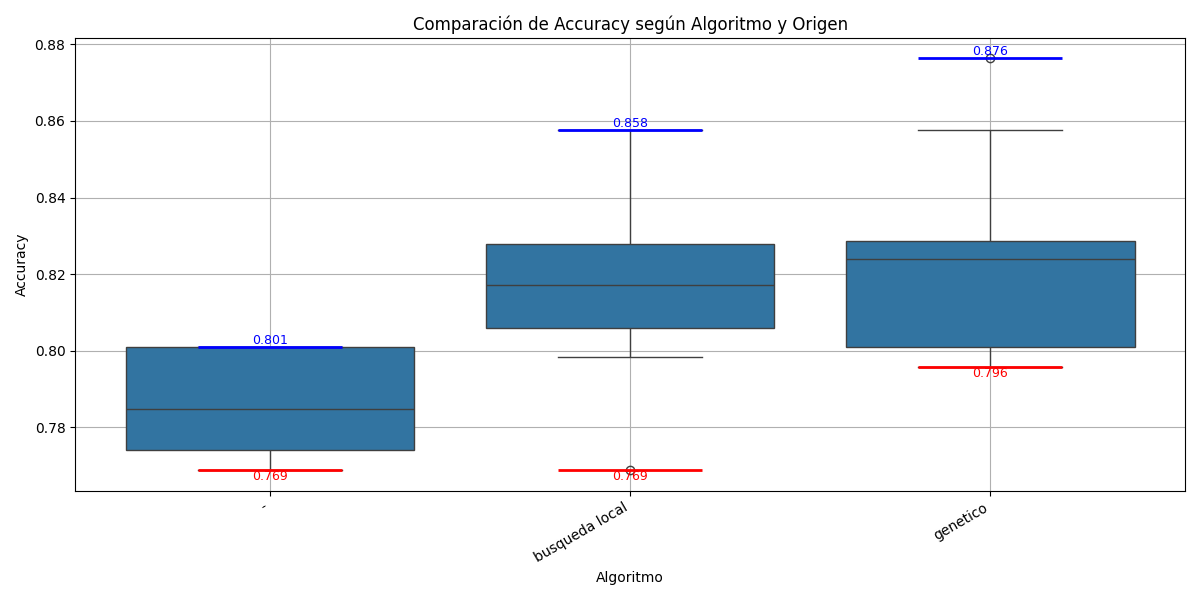
\includegraphics[width=1\textwidth]{imagenes/evaluaciones/comparacion_bl-gen_v1}
    \caption{Boxplot comparando la búsqueda local con el algoritmo genético v1 usando \textit{accuracy}.}
    \label{fig:bl-vs-gen-v1}
\end{figure}

Tal como se observa en la Figura~\ref{fig:bl-vs-gen-v1}, el algoritmo genético consigue una mediana de \textbf{accuracy} más alta que la búsqueda local,
reflejando un rendimiento medio más consistente.
Además, presenta un valor máximo superior (alcanza hasta \textbf{0.876}), lo que evidencia su mayor potencial para encontrar soluciones de alta calidad.

No obstante, también se aprecia una ligera mayor dispersión en los resultados del algoritmo genético, particularmente hacia los valores bajos.
Esto indica que, pese a su capacidad exploratoria, el genético puede generar soluciones poco efectivas si no se controlan adecuadamente ciertos operadores como el cruce o la mutación.
De hecho, su valor mínimo (\textbf{0.796}) es superior al de la búsqueda local en esta comparativa, pero deja margen para mejoras en la presión selectiva o en mecanismos que eviten estancamientos.

\colorbox{yellow}{¿Sobra el siguiente apartado?}
La búsqueda local, por su parte, mantiene un comportamiento más estable, aunque con una mediana ligeramente inferior.
Su distribución es más concentrada y limitada en el extremo superior, lo que evidencia su carácter más explotador pero con menor capacidad para alcanzar soluciones óptimas globales.

Estos resultados sirvieron como evidencia empírica para continuar desarrollando nuevas versiones del algoritmo genético,
incorporando mejoras específicas en sus operadores con el fin de aprovechar su capacidad exploratoria y, al mismo tiempo, mitigar sus limitaciones.

\section{Modificando el operador de cruce}\label{sec:incorporacion-cruce}
La primera mejora introducida fue en el operador de cruce.
En lugar del cruce aleatorio clásico, se implementó un cruce ponderado que tiene en cuenta el fitness de los progenitores para asignar más peso a las contribuciones del mejor.
Esta mejora se aplicó en la Versión 2 del algoritmo (ver \hyperref[sec:genetico-v2]{Sección~\ref*{sec:genetico-v2}}).
Además, se introdujo un criterio selectivo adicional: de los dos hijos generados, solo se conservaba el mejor.
Esta modificación redujo la dispersión de los resultados y aceleró la convergencia del algoritmo, permitiendo heredar más eficazmente características prometedoras y evitando que soluciones débiles dominaran el proceso evolutivo.

\section{Modificación del operador de mutación}\label{sec:modificacion-mutacion}
En paralelo a la mejora del cruce, también se revisó la estrategia de mutación.
La versión original usaba una tasa fija del 10\% sobre el subconjunto de imágenes seleccionadas:
$$
    num_swaps=max(1,lengthx0.1)
$$
Sin embargo, esta regla podía resultar demasiado agresiva o demasiado limitada dependiendo del tamaño del subconjunto.
Por ello, se adoptó una nueva fórmula más adaptativa:

$$
    num_swaps=min(lengthx0.15,lengthx0.8)
$$
...
$$
    num_swaps=min(lengthx0.15,lengthxratiox0.8)
$$
Esta versión ajusta automáticamente el número de intercambios en función del tamaño relativo del subconjunto mutado, favoreciendo un equilibrio más eficaz entre exploración y estabilidad.

\section{Incorporación del reinicio poblacional}\label{sec:incorporacion-reinicio-poblacional}
En la Versión 3 del algoritmo (ver \hyperref[sec:genetico-v3]{Sección~\ref*{sec:genetico-v3}}) se incorporó una lógica de reinicio poblacional.
El algoritmo monitoriza el comportamiento del segundo mejor individuo, y si este no mejora en dos generaciones consecutivas, se reinicia parcialmente la población manteniendo solo el mejor individuo.
Esta estrategia resultó muy útil para escapar de óptimos locales, introduciendo diversidad controlada sin perder el conocimiento acumulado.
El reinicio ayudó a reactivar la evolución en ejecuciones que de otro modo quedaban estancadas, mejorando tanto los resultados máximos como la estabilidad entre ejecuciones.

\section{Incorporación de versiones libres}\label{sec:incorporacion-versiones-libres}
Finalmente, se exploraron variantes "libres" del algoritmo, permitiendo que el número de imágenes seleccionadas evolucionara dinámicamente.
Al activar el parámetro adjust\_size, el operador de cruce genera subconjuntos cuyo tamaño varía entre el 50\% y el 150\% del tamaño base.
Esta flexibilidad estructural permite al algoritmo ajustar de forma estocástica la escala de las soluciones, adaptándose mejor a la complejidad del problema.
Las versiones libres demostraron una mejora en diversidad poblacional y una mayor capacidad de ajuste, especialmente en casos donde no se conoce a priori el tamaño óptimo del subconjunto de entrenamiento.

\section{Evaluación del algoritmo memético}\label{sec:evaluacion-algoritmo-memetico}
Finalmente, se evaluó el algoritmo memético (ver \hyperref[sec:algoritmo-memetico]{Sección~\ref*{sec:algoritmo-memetico}}) el cual combina la evolución genética con una búsqueda local probabilística.
Esta técnica híbrida fue capaz de generar subconjuntos altamente representativos, superando a las versiones iniciales del genético tanto en precisión como en robustez de los resultados.

Se incluyó también una variante libre del algoritmo (\hyperref[subsec:memetico-libre]{Apartado~\ref*{subsec:memetico-libre}}) que introdujo flexibilidad adicional en el tamaño de las soluciones y en la exploración local.
Aunque con un coste computacional algo mayor, estas versiones ofrecieron una de las mejores combinaciones entre rendimiento y estabilidad.

\section{Comparación final entre enfoques}\label{sec:comparacion-final-enfoques}
En esta sección se realiza una comparación conjunta entre todos los algoritmos implementados.
Se presentan boxplots y gráficos de barras que muestran la evolución del accuracy, el porcentaje de datos utilizados y el equilibrio entre clases.

Los algoritmos meméticos y genéticos v2/v3 (especialmente en sus versiones libres) destacan como los más eficaces, consiguiendo una reducción significativa del conjunto de entrenamiento sin penalizar la precisión.
Además, se observa una menor varianza en sus resultados, lo que indica una mayor consistencia entre ejecuciones.

\section{Validación con el dataset PAINTING}\label{sec:validacion-con-painting}
Para comprobar la generalización de los algoritmos, se repitieron los experimentos con el dataset PAINTING.
Este conjunto presenta mayor complejidad tanto en número de clases como en diversidad visual.
A pesar de ello, los algoritmos avanzados lograron mantener un rendimiento competitivo, confirmando su aplicabilidad en contextos más exigentes.